% http://www.idsc.ethz.ch/education/theses-semester-projects.html
% IDSC LaTeX Thesis Template
% 
% Author(s):	Eric Müller
% 				Institute for Dynamic Systems and Control
% 				Swiss Federal Institute of Technology (ETH) Zurich
% 
% Created:		2004/04/02  (Eric Mueller)
% 
% Notes: Has been tested on Windows 7 + MikTeX + TeXnicCenter
%
% Revisions: 	2009/05/29  (Soren Ebbesen)
% 				    2011/03/22	(Soren Ebbesen)
%             2013/03/08	(Soren Ebbesen)
%             2014/03/13	(Soren Ebbesen)
% ______________________________________________________________________________
\documentclass[10pt,twoside,a4paper,fleqn]{report}

%custom commands for comments of Supervisor (sv), phd candidate(pc)
\newcommand{\sv}[1]{\textcolor{red}{{\bf SV:}~#1}}    
\newcommand{\pc}[1]{\textcolor{cyan}{{\bf PC:}~#1}} 

\usepackage[english,mt]{ethidsc} % Special IDSC styles and commands      	
								 % {german}/english: language of headings, etc.
								 % {st}/bt/mt: {semester}/bachelor/master thesis
\usepackage{caption, subcaption}
% Image position [H]
\usepackage{float} % table position
%\usepackage{csvsimple} %(if want to add tables from csv. Otherwise use: https://www.tablesgenerator.com/latex_tables and import them from File->import csv file...)
% Tables with cells that take multiple rows
\usepackage{multirow}
% Allow for a new line in the same cell of a table (https://tex.stackexchange.com/questions/2441/how-to-add-a-forced-line-break-inside-a-table-cell/19678)
\usepackage{makecell}
% text color
\usepackage{xcolor}
% forests (used to represent classes in the code)
\usepackage[edges]{forest}
% forests (attempt II)
\usepackage{forest}
% acronym
\usepackage{acronym}
% to include a pdf with the title page
\usepackage{pdfpages}

\usetikzlibrary{arrows.meta}
\forestset{
  dir tree/.style={
    for tree={
      parent anchor=south west,
      child anchor=west,
      anchor=mid west,
      inner ysep=1pt,
      grow'=0,
      align=left,
      edge path={
        \noexpand\path [draw, \forestoption{edge}] (!u.parent anchor) ++(1em,0) |- (.child anchor)\forestoption{edge label};
      },
      font=\sffamily,
      if n children=0{}{
        delay={
          prepend={[,phantom, calign with current]}
        }
      },
      fit=band,
      before computing xy={
        l=2em
      }
    },
  }
}
% accents and special characters
%\usepackage[utf8]{inputenc}

% Page header (don't change)________________________________________________
\setlength{\parindent}{0em}                 % Disable parindent
\rhead[\nouppercase{\rightmark}]{\thepage}  % Special headings
\lhead[\thepage]{\nouppercase{\leftmark}}   % Special headings
\cfoot{}                                    % Special headings


% Title page (please fill in)____________________________________________
\title{Configuring networks on neuromorphic hardware}


\studentA{Dmitrii Zendrikov}
\ethidA{}
\semesterA{}
\emailA{dmitrii@ini.uzh.ch}


\supervision{Prof. Dr. Giacomo Indiveri\\Dr. Matthew Cook\\Dr. Yulia Sandamirskaya}
\date{November 2022}
%\type{Ph.D. Thesis}
%\identification{IDSC-XX-YY-ZZ} 		% Project identifier

\infopage
%\declaration


% Begin document___________________________________________________________
\begin{document}
\maketitle 							% Create title page


\newlength{\originalVOffset}
 \newlength{\originalHOffset}
 \setlength{\originalVOffset}{\voffset}   
 \setlength{\originalHOffset}{\hoffset}
 \setlength{\voffset}{0cm}
 \setlength{\hoffset}{0cm}
 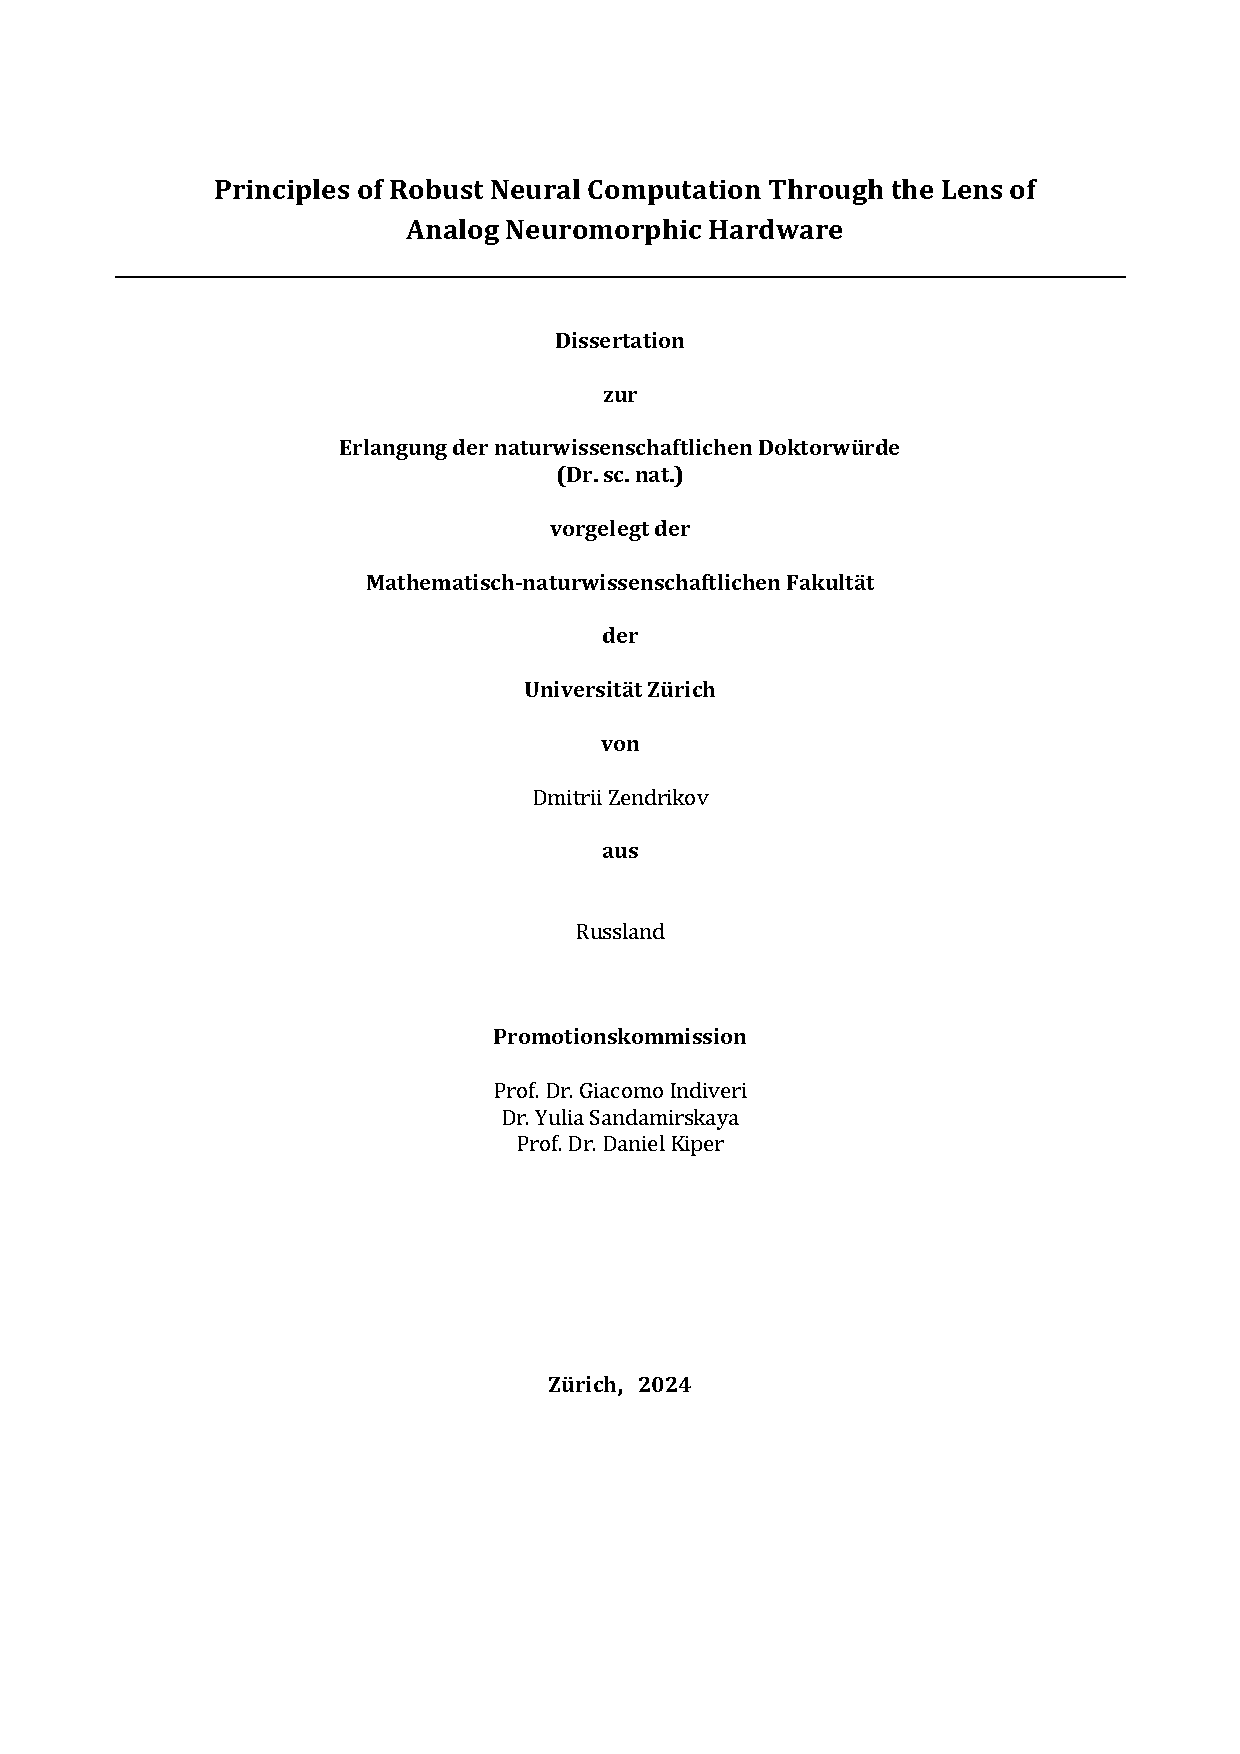
\includepdf[pages=-]{Titelblatt.pdf}
 \setlength{\voffset}{\originalVOffset}
 \setlength{\hoffset}{\originalHOffset}
 
% Preamble_______________________________________________________________

\pagenumbering{roman} 				% Begin roman page numbering (i,ii,...)

%---------------------------------------------------------------------------
% Preface

\chapter*{Abstract}
 \addcontentsline{toc}{chapter}{Abstract}

Neuromorphic electronics provide a computational substrate that natively supports spiking neural networks through device physics, making them strong competitors for low-power edge computing applications. This class of devices is fundamentally different from conventional digital processors, and so is the computation they are capable of.

Development path of this technology is about to reach a new stage, combining multiple domains, like CMOS circuits and memristive or ferroelectric devices, on the same die. To educate the upcoming design choices, it is necessary to build a firm understanding of the advantages and limitations of the current generation of chips, which can be done by systematically extracting the most out of them and identifying missing components for possible applications.

This work represents a bottom-up journey of scientific exploration towards achieving robust neuromorphic computing. Having the dream of autonomous intelligent neuromorphic systems as a distant goal, we define and test computational primitives serving as building blocks for such intelligence. We use a current-generation general-purpose neuromorphic processor to demonstrate the accessibility of computational elements, previously implemented with application-specific circuits. Moreover, since the chip design is inspired by the nervous system at the lowest level, we demonstrate that the brain-derived strategies benefit coding and its robustness at the network level.

Through analysis of individual neuron circuits, small populations and the exploitation of the reprogrammable routing scheme of the chip, we configure multiple network prototypes that implement i) a network of relations, ii) a model of unsupervised cortical map formation, iii) a spatiotemporal pattern classifier and iv) an example of closed-loop neuromorphic agent capable of reinforcement learning.

As a result, we provide tools and insights into how neuromorphic hardware should be approached, showing how such seemingly different domains of computation, in fact, fit well under the umbrella of the same principles of space and time averaging, and introduced stochasticity.


%\dz{DRAFT: Understanding by building is really the epitome of this work. While the tangible global task declared for the project had been to "build neuromorphic agents", it was formulated in a way that fosters bio-inspired methodological search, drastically constraining the field of possible solutions. This work represents the work philosophy and the results of what happens, when instead of paving a high-level path to a problem solution, one would rather focus on low-level details, crossing out some technologies and keeping the others, resulting in a small piece of this "edible pie" in the end, the intersection of all constraints. And only then, having this set of rules declared important, you begin to see what high-level task it would solve. This probably tells the story of a true bottom-up approach, spanning across multiple domains and converging to a functional prototype.}
\newpage
 
\chapter*{Acknowledgements}
\addcontentsline{toc}{chapter}{Acknowledgements}

This work is supported by the EU ERC Grant 'NeuroAgents' (No. 724295)

%\begin{verbatim}
%thesis thanks:
%Giacomo for care, believing in me, and the art of scientific storytelling, the example of
%    passion for the elegance of neuromorphic technology
%my dad and family
%Kathrin and Simone, not only administrative, but emotional support
%Sergio (and Sonia) - for work discussions but also hospitality and good times on Sardinia
%Alexander Paraskevov
%NCS Group
%Nicoletta 
%Eugenia
%Karina
%Veronika 
%Yulia for the inspiration to push and leading by example. And of course aviation
%Hector for making me rebuild my mental health by reintegrating me into zurich music %scene
%Maryada
%Matteo
%Moritz for setting a bar and an example, how to work and how to party. And CapoCaccia and Kafischnaps sessions
%Matthew Cook
%Vanessa (for sparkle and energy)
%Leo for assuming i have all the answers and making me try to live up to expectations
%Ayush
%Alex & UW
%Sasha
%    
%\end{verbatim}
\newpage

%---------------------------------------------------------------------------
% Table of contents

 \setcounter{tocdepth}{2}
 \tableofcontents

 \newpage

%---------------------------------------------------------------------------
% Symbols

\chapter*{Nomenclature}\label{chap:symbole}
 \addcontentsline{toc}{chapter}{Nomenclature}

\section*{Acronyms and Abbreviations}
\begin{acronym}
\acro{ADC}[ADC]{Analog to Digital Converter}
\acro{ADEXP}[AdExp-I\&F]{Adaptive-Exponential Integrate and Fire}
\acro{ADM}[ADM]{Asynchronous Delta Modulator}
\acro{AER}[AER]{Address-Event Representation}
\acro{AEX}[AEX]{AER EXtension board}
\acro{AE}[AE]{Address-Event}
\acro{AFM}[AFM]{Atomic Force Microscope}
\acro{AGC}[AGC]{Automatic Gain Control}
\acro{AI}[AI]{Artificial Intelligence}
\acro{AMDA}[AMDA]{AER Motherboard with D/A converters}
\acro{ANN}[ANN]{Artificial Neural Network}
\acro{API}[API]{Application Programming Interface}
\acro{APMOM}[APMOM]{Alternate Polarity Metal On Metal}
\acro{ARM}[ARM]{Advanced RISC Machine}
\acro{ASIC}[ASIC]{Application Specific Integrated Circuit}
\acro{AdExp}[AdExp-IF]{Adaptive Exponential Integrate-and-Fire}
\acro{BCM}[BMC]{Bienenstock-Cooper-Munro}
\acro{BD}[BD]{Bundled Data}
\acro{BEOL}[BEOL]{Back-end of Line}
\acro{BG}[BG]{Bias Generator}
\acro{BMI}[BMI]{Brain-Machince Interface}
\acro{BTB}[BTB]{band-to-band tunnelling}
\acro{CAD}[CAD]{Computer Aided Design}
\acro{CAM}[CAM]{Content Addressable Memory}
\acro{CAVIAR}[CAVIAR]{Convolution AER Vision Architecture for Real-Time}
\acro{CA}[CA]{Cortical Automaton}
\acro{CCN}[CCN]{Cooperative and Competitive Network}
\acro{CDR}[CDR]{Clock-Data Recovery}
\acro{CFC}[CFC]{Current to Frequency Converter}
\acro{CHP}[CHP]{Communicating Hardware Processes}
\acro{CMIM}[CMIM]{Metal-insulator-metal Capacitor}
\acro{CML}[CML]{Current Mode Logic}
\acro{CMOL}[CMOL]{Hybrid CMOS nanoelectronic circuits}
\acro{CMOS}[CMOS]{Complementary Metal-Oxide-Semiconductor}
\acro{CNN}[CCN]{Convolutional Neural Network}
\acro{COTS}[COTS]{Commercial Off-The-Shelf}
\acro{CPG}[CPG]{Central Pattern Generator}
\acro{CPLD}[CPLD]{Complex Programmable Logic Device}
\acro{CPU}[CPU]{Central Processing Unit}
\acro{CSM}[CSM]{Cortical State Machine}
\acro{CSP}[CSP]{Constraint Satisfaction Problem}
\acro{CTXCTL}[CTXCTL]{CortexControl}
\acro{CV}[CV]{Coefficient of Variation}
\acro{DAC}[DAC]{Digital to Analog Converter}
\acro{DAS}[DAS]{Dynamic Auditory Sensor}
\acro{DAVIS}[DAVIS]{Dynamic and Active Pixel Vision Sensor}
\acro{DBN}[DBN]{Deep Belief Network}
\acro{DFA}[DFA]{Deterministic Finite Automaton}
\acro{DIBL}[DIBL]{drain-induced-barrier-lowering}
\acro{DI}[DI]{delay insensitive}
\acro{DMA}[DMA]{Direct Memory Access}
\acro{DNF}[DNF]{Dynamic Neural Field}
\acro{DNN}[DNN]{Deep Neural Network}
\acro{DOF}[DOF]{Degrees of Freedom}
\acro{DPE}[DPE]{Dynamic Parameter Estimation}
\acro{DPI}[DPI]{Differential Pair Integrator}
\acro{DRAM}[DRAM]{Dynamic Random Access Memory}
\acro{DRRZ}[DR-RZ]{Dual-Rail Return-to-Zero}
\acro{DR}[DR]{Dual Rail}
\acro{DSP}[DSP]{Digital Signal Processor}
\acro{DVS}[DVS]{Dynamic Vision Sensor}
\acro{DYNAP}[DYNAP]{Dynamic Neuromorphic Asynchronous Processor}
\acro{EBL}[EBL]{Electron Beam Lithography}
\acro{EDVAC}[EDVAC]{Electronic Discrete Variable Automatic Computer}
\acro{EEG}[EEG]{electroencephalography}
\acro{EIN}[EIN]{Excitatory-Inhibitory Network}
\acro{EM}[EM]{Expectation Maximization}
\acro{EPSC}[EPSC]{Excitatory Post-Synaptic Current}
\acro{EPSP}[EPSP]{Excitatory Post-Synaptic Potential}
\acro{EZ}[EZ]{Epileptogenic Zone}
\acro{FDSOI}[FDSOI]{Fully-Depleted Silicon on Insulator}
\acro{FET}[FET]{Field-Effect Transistor}
\acro{FFT}[FFT]{Fast Fourier Transform}
\acro{FI}[F-I]{Frequency-Current}
\acro{FPGA}[FPGA]{Field Programmable Gate Array}
\acro{FR}[FR]{Fast Ripple}
\acro{FSA}[FSA]{Finite State Automaton}
\acro{FSM}[FSM]{Finite State Machine}
\acro{GIDL}[GIDL]{gate-induced-drain-leakage}
\acro{GOPS}[GOPS]{Giga-Operations per Second}
\acro{GPU}[GPU]{Graphical Processing Unit}
\acro{GUI}[GUI]{Graphical User Interface}
\acro{HAL}[HAL]{Hardware Abstraction Layer}
\acro{HFO}[HFO]{High Frequency Oscillation}
\acro{HH}[H\&H]{Hodgkin \& Huxley}
\acro{HMM}[HMM]{Hidden Markov Model}
\acro{HRS}[HRS]{High-Resistive State}
\acro{HR}[HR]{Human Readable}
\acro{HSE}[HSE]{Handshaking Expansion}
\acro{HW}[HW]{Hardware}
\acro{ICT}[ICT]{Information and Communication Technology}
\acro{IC}[IC]{Integrated Circuit}
\acro{IEEG}[iEEG]{intracranial electroencephalography}
\acro{IF2DWTA}[IF2DWTA]{Integrate \& Fire 2--Dimensional WTA}
\acro{IFSLWTA}[IFSLWTA]{Integrate \& Fire Stop Learning WTA}
\acro{IF}[I\&F]{Integrate-and-Fire}
\acro{IMU}[IMU]{Inertial Measurement Unit}
\acro{INCF}[INCF]{International Neuroinformatics Coordinating Facility}
\acro{INI}[INI]{Institute of Neuroinformatics}
\acro{IO}[I/O]{Input/Output}
\acro{IPSC}[IPSC]{Inhibitory Post-Synaptic Current}
\acro{IPSP}[IPSP]{Inhibitory Post-Synaptic Potential}
\acro{IP}[IP]{Intellectual Property}
\acro{ISI}[ISI]{Inter-Spike Interval}
\acro{IoT}[IoT]{Internet of Things}
\acro{JFLAP}[JFLAP]{Java - Formal Languages and Automata Package}
\acro{LEDR}[LEDR]{Level-Encoded Dual-Rail}
\acro{LFP}[LFP]{Local Field Potential}
\acro{LLC}[LLC]{Low Leakage Cell}
\acro{LNA}[LNA]{Low-Noise Amplifier}
\acro{LPF}[LPF]{Low Pass Filter}
\acro{LRS}[LRS]{Low-Resistive State}
\acro{LSM}[LSM]{Liquid State Machine}
\acro{LTD}[LTD]{Long Term Depression}
\acro{LTI}[LTI]{Linear Time-Invariant}
\acro{LTP}[LTP]{Long Term Potentiation}
\acro{LTU}[LTU]{Linear Threshold Unit}
\acro{LUT}[LUT]{Look-Up Table}
\acro{LVDS}[LVDS]{Low Voltage Differential Signaling}
\acro{MCMC}[MCMC]{Markov-Chain Monte Carlo}
\acro{MEMS}[MEMS]{Micro Electro Mechanical System}
\acro{MFR}[MFR]{Mean Firing Rate}
\acro{MIM}[MIM]{Metal Insulator Metal}
\acro{MLP}[MLP]{Multilayer Perceptron}
\acro{MOSCAP}[MOSCAP]{Metal Oxide Semiconductor Capacitor}
\acro{MOSFET}[MOSFET]{Metal Oxide Semiconductor Field-Effect Transistor}
\acro{MOS}[MOS]{Metal Oxide Semiconductor}
\acro{MRI}[MRI]{Magnetic Resonance Imaging}
\acro{NDFSM}[NDFSM]{Non-deterministic Finite State Machine} 
\acro{ND}[ND]{Noise-Driven}
\acro{NEF}[NEF]{Neural Engineering Framework}
\acro{NHML}[NHML]{Neuromorphic Hardware Mark-up Language}
\acro{NIL}[NIL]{Nano-Imprint Lithography}
\acro{NMDA}[NMDA]{N-Methyl-D-Aspartate}
\acro{NME}[NE]{Neuromorphic Engineering}
\acro{NN}[NN]{Neural Network}
\acro{NOC}[NoC]{Network-on-Chip}
\acro{NRZ}[NRZ]{Non-Return-to-Zero}
\acro{NSM}[NSM]{Neural State Machine}
\acro{OR}[OR]{Operating Room}
\acro{OTA}[OTA]{Operational Transconductance Amplifier}
\acro{PCB}[PCB]{Printed Circuit Board}
\acro{PCHB}[PCHB]{Pre-Charge Half-Buffer}
\acro{PCM}[PCM]{Phase Change Memory}
\acro{PE}[PE]{Phase Encoding}
\acro{PFA}[PFA]{Probabilistic Finite Automaton}
\acro{PFC}[PFC]{prefrontal cortex}
\acro{PFM}[PFM]{Pulse Frequency Modulation}
\acro{PR}[PR]{Production Rule}
\acro{PSC}[PSC]{Post-Synaptic Current}
\acro{PSP}[PSP]{Post-Synaptic Potential}
\acro{PSTH}[PSTH]{Peri-Stimulus Time Histogram}
\acro{QDI}[QDI]{Quasi Delay Insensitive}
\acro{RAM}[RAM]{Random Access Memory}
\acro{RA}[RA]{Resected Area}
\acro{RDF}[RDF]{random dopant fluctuation}
\acro{RELU}[ReLu]{Rectified Linear Unit}
\acro{RLS}[RLS]{Recursive Least-Squares}
\acro{RMSE}[RMSE]{Root Mean Squared-Error}
\acro{RMS}[RMS]{Root Mean Squared}
\acro{RNN}[RNN]{Recurrent Neural Networks}
\acro{ROLLS}[ROLLS]{Reconfigurable On-Line Learning Spiking}
\acro{RRAM}[R-RAM]{Resistive Random Access Memory}
\acro{R}[R]{Ripples}
\acro{SAC}[SAC]{Selective Attention Chip}
\acro{SAT}[SAT]{Boolean Satisfiability Problem}
\acro{SCX}[SCX]{Silicon CorteX}
\acro{SD}[SD]{Signal-Driven}
\acro{SEM}[SEM]{Spike-based Expectation Maximization}
\acro{SLAM}[SLAM]{Simultaneous Localization and Mapping}
\acro{SNN}[SNN]{Spiking Neural Network}
\acro{SNR}[SNR]{Signal to Noise Ratio}
\acro{SOC}[SOC]{System-On-Chip}
\acro{SOI}[SOI]{Silicon on Insulator}
\acro{SOZ}[SOZ]{Seizure Onset Zone}
\acro{SP}[SP]{Separation Property}
\acro{SRAM}[SRAM]{Static Random Access Memory}
\acro{STDP}[STDP]{Spike-Timing Dependent Plasticity}
\acro{STD}[STD]{Short-Term Depression}
\acro{STP}[STP]{Short-Term Plasticity}
\acro{STT-MRAM}[STT-MRAM]{Spin-Transfer Torque Magnetic Random Access Memory}
\acro{STT}[STT]{Spin-Transfer Torque}
\acro{SW}[SW]{Software}
\acro{TCAM}[TCAM]{Ternary Content-Addressable Memory}
\acro{TFT}[TFT]{Thin Film Transistor}
\acro{TLE}[TLE]{Temporal Lobe Epilepsy}
\acro{USB}[USB]{Universal Serial Bus}
\acro{VHDL}[VHDL]{VHSIC Hardware Description Language}
\acro{VLSI}[VLSI]{Very Large Scale Integration}
\acro{VOR}[VOR]{Vestibulo-Ocular Reflex}
\acro{WCST}[WCST]{Wisconsin Card Sorting Test}
\acro{WTA}[WTA]{Winner-Take-All}
\acro{XML}[XML]{eXtensible Mark-up Language}
\acro{divmod3}[DIVMOD3]{divisibility of a number by three}
\acro{hWTA}[hWTA]{hard Winner-Take-All}
\acro{sWTA}[sWTA]{soft Winner-Take-All}
\end{acronym}



 \newpage

%---------------------------------------------------------------------------


\pagestyle{fancy}               	% Fancy headings
\pagenumbering{arabic}				% Begin arabic page numbering (1,2,...)



% Chapters______________________________________________________________________


\chapter{Introduction}
\label{chapter:introduction}

%\subsection{Thesis Objectives}
\section{Thesis Outline}

\subsection{Making neuromorphic hardware more accessible(??)}

\newpage

\input{chapters/2_Modeling_and_emulation.tex}
\newpage

\chapter{Signal representation in neural systems}
\label{ch:signal_represetations}


\section{Neural coding strategies. Single neuron dynamics}
\section{Population coding, averaging across space}
\section{Temporal averaging, spike integration}
\section{Temporal signal representation, internal dynamics and states}

\newpage

\chapter{Neuromorphic DYNAP-SE1 chip: properties, benefits, limitations, links to biology}
\label{ch:neuromorphic_harware}


\section{Chip architecture}

-- Mixed-signal: Analog asynchronous neuron\\synapse circuits, digital hierarchical routing
-- Shared parameters withing each core

\section{Behaviour characterization: strategies and results}
\subsection{Waveform capture and analysis}
\subsection{Setting biases}
\subsection{Mismatch and noise effects scale}

-- Introduce mismatch and noise as concepts


\subsection{Achieving EI balance on the chip (?)}
\newpage

\chapter{Relational networks (??)}
\label{ch:Relational_networks}

\section{Concept}

\section{Results}
\newpage

\chapter{Learning strategies and implementation with neuromorphic hardware}
\label{ch:Plasticity_and_learning}

\section{Approaches to learning with hardware: local vs global, supervised vs unsupervised, weight transfer vs in-the-loop}

\subsection{RNN Transfer learning (SGD implementation example)}

\subsection{Chip-in-the-loop learning (to account for exact mismatch profile)}

\section{Hardware-friendly implementation details}
\subsection{Weight quantization}
\subsection{Batched weight updates}

\newpage

\chapter{On-Chip Network prototypes}
\label{ch:temporal_decoding_prototype}

\section{Clustered Winner-Take-All}
\subsection{Signal processing capabilities}
\subsection{Network capacity}
\subsection{Selective amplification}

\section{WTA and Plasticity. Unsupervised map learning}

\section{Adaptive target following with reinforcement learning (full hardware setup, Caterina's project)}

\section{Spatiotemporal pattern recognition prototype with delay lines}

https://ieeexplore.ieee.org/document/5173584

\section{Discussion: applications and future development}
\newpage

\chapter{Final thoughts}
\label{ch:conclusion}

\section{Spike timing matters}

\section{Spiking networks are yet to find (their own domain of) application}

SNNs are a separate operational system to ANNs, therefore the benchmarks should not be directly applied, they should not compete

\section{Future work: self organizing arbitrary length delaylines with local rules}
\newpage

% Appendix______________________________________________________________________
\appendix
 \chapter{PyGetScope Tool}
 \label{appendix:pyscope}
\pyobject{PyGetScope} is a Python tool for interaction with Agilent 4000x and 6000x series oscilloscopes~\cite{pygetscope}. It is a Python wrapper that uses \pyobject{pyvisa} library, sending SCPI commands and receiving data from devices allowing automated remote operation. Full functionality of this library is listed below. For installation and configuration instructions, please refer to the repository ReadMe section.\\

\textbf{Link:} \url{https:/code.ini.uzh.ch/ncs/libs/pygetscope}

\section{Initialization}

The class is imported in a standard way, allowing interaction with the scope through a \verb|PyScope| object:

\begin{lstlisting}[language=Python, caption=PyScope module initialization]
from pygetscope.py_scope import PyScope
my_scope = PyScope()
\end{lstlisting}


\section{Waveform acquisition}

The core function \verb|get_waveform(|\verb|channel_id|, \verb|[num_points=1000, instant_plot=False|, \verb|keep_running=True])| of the \verb|PyScope| class returns a \pyobject{NumPy} array of data points in the format \verb|[timestamp, voltage]|, present in the currently visible screen area given the set vertical and horizontal scales and offsets.\\

Additional arguments allow extended functionality:
\begin{itemize}
    \item \verb|num_points=[1000 .. 20000]| sets the number of datapoints returned by the scope. For values higher than 1000 the \verb|keep_running| argument is set to \verb|False| as the connection bandwidth becomes an issue 
    \item \verb|instant_plot=[True\False]| immediately returns a \pyobject{PyPlot} of the recorded waveform
    \item \verb|keep_running=[True\False]| sets if the oscilloscope should stop after the acquisition of the waveform (for extraction of synchronized waveforms from multiple channels)
\end{itemize}


\section{Controlling the oscilloscope}

The rest of the library functionality contains tools to control the vertical and horizontal scales of the input signals, vertical offsets and the trigger. The \textbf{SET} functions pass apply the new values of the parameters, and the \textbf{GET} return the current values. If any of the physical knobs are turned on the device, the returned values would reflect that.

\subsection*{Scaling}

\textbf{SET} functions:
\begin{itemize}
    
    \item \verb|set_timescale()| set the time scale in seconds
    \item \verb|set_timebase_pos()| sets the horizontal offset of the waveform
    \item \verb|set_channel_scale(channel_id, scale)| sets the vertical scale for the selected channel in volts
    \item \verb|set_channel_offset(channel_id, scale)| sets the offset scale for the selected channel
    \item \verb|autoscale()| enables the built-in autoscaling routine of the device. Equivalent to the physical Autoscale button.
    \item \verb|find_offset(channel_id)| is a custom procedure that finds \textbf{both} vertical \textbf{scale} and \textbf{offset} that make the channel waveform fit the screen area

\end{itemize}

\noindent\textbf{GET} functions:

\begin{itemize}
    
    \item \verb|get_timescale()| returns the current scale in seconds
    \item \verb|get_timebase_pos()| returns the current horizontal offset of the waveform
    \item \verb|get_channel_scale(channel_id)| returns the current vertical scale for the selected channel in volts
    \item \verb|get_channel_offset(channel_id)| returns the current offset scale for the selected channel

\end{itemize}

\subsection*{Channel visibilty}

A set of functions for showing or hiding selected channels.

\begin{itemize}
    
    \item \verb|show_channel(channel_id)| enables measurement and display from the selected channel
    \item \verb|hide_channel(channel_id)| disables the selected channel
    \item \verb|hide_all_channels()| disables all input channels

\end{itemize}

\subsection*{Trigger}

A set of functions for operating the trigger for the periodic signals.\\

\noindent\textbf{SET} functions:

\begin{itemize}
    
    \item \verb|set_trigger_source(channel_id)| sets which channel should serve as a source for the trigger
    \item \verb|set_trigger_level(voltage)| sets the voltage level for the trigger

\end{itemize}

\noindent\textbf{GET} functions:

\begin{itemize}
    
    \item \verb|get_trigger_source()| returns the ID of the channel the trigger is currently used for
    \item \verb|get_trigger_level()| returns the level of the trigger

\end{itemize}

\subsection*{Operational}

A set of functions controlling the overall operation mode of the device

\begin{itemize}
    
    \item \verb|run()| enables continuous acquisition of the currently enabled (shown) channels
    \item \verb|stop()| stops data acquisition, freezing the state of the shown waveforms within the screen area. Vertical and horizontal offsetting of the visible waveform pieces is still possible in this state.

\end{itemize}

\subsection*{Lower level access}

\textit{Warning: use with caution as not all devices accept all of the SCPI commands. Sending wrong commands might lead to the bus being stuck, requiring device reboot.}\\

Functions for passing custom SCPI commands through. Both functions accept a string that is passed to the oscilloscope. The only difference between the query and the command is the expectation of returned data in case of the former.

\begin{itemize}
    
    \item \verb|do_command(command)| passes an SCPI command string to the device
    \item \verb|do_query_string(query)| passes an SCPI query to the device, returning the response, and checks for any pending readback errors, as the pending errors might jam the output for any future queries. In case of the error, raises an exception with the error code.

\end{itemize}

  \chapter{Bias Tuning Tools}
 \label{appendix:bias_tuning_tools}

\textbf{Link:} \url{}

 \textit{Warning:} Currently, the entire package is written for CTXCTL and needs converting for Samna support.\\

 The procedure for bias configuration, however, still applies:

 \url{https://code.ini.uzh.ch/ncs/libs/dynap-se1/-/blob/main/dynapse-biases-howtosetup.md}
 
 \chapter{Appendix C: DYNAP-SE Visualization and interactive control tools}
 \label{appendix:bias_tuning_tools}
 \chapter{Appendix D: Network Primitives for DYNAP-SE1}
 \label{appendix:bias_tuning_tools}

 \section{Clustered WTA class reference}

 \section{Reward-gated STDP class reference}

 \section{Delay chain class reference}


% Bibliography__________________________________________________________________
% Literature (Additional references can be added to the .bib-file manually, or by using, for example, the free application JabRef). Compile in the following order: latex -bibtex -latex -latex

\bibliographystyle{plain}
\bibliography{biblio/biblioncs}

\end{document}
